\documentclass{article}
\usepackage{listings}
\usepackage[margin=1in]{geometry}
\usepackage{graphicx}
\usepackage{amsmath}
\usepackage[ruled,vlined]{algorithm2e}


\title{CMOR 421/521, Homework \#2: \LaTeX{} Submission}
\author{\texttt{amc50}}
\date{March 26, 2024}

\begin{document}
\maketitle

\section{Compilation}
\subsection{Accessing NOTS Cluster}
All of the following processes and results were run on the NOTS Cluster. It is also import to note that in order to complete a thorough evaluation on the influence of matrix size and thread number on the performance of each implementation, multiple executions of the following compilation commands were required. The reason that this is the case is because the cluster would continually kill the job, likely due to the request for 32 CPUs exceeding the resource limit. To mitigate the inconvenience of having to repeatedly execute the commands there are a few potential alternative approaches. The first is to simply reduce the requested CPUs and rely on hyper-threading to meet thread requirements. The other option is to run on the local desktop which is somewhat slower but will not kick off from the node so is more convenient. For running on the local desktop the Makefile does need to be slightly adjusted as the compilation command used is different. For my local MacBook the command used on NOTS to compile of \texttt{g++} defaults to clang which does not support \texttt{-fopenmp} requiring \texttt{g++-13} to be specified to resolve this issue. For the NOTS cluster, \texttt{g++} is adequate and what is included in the provided code. Regardless, for the all the following NOTS was used and the compilation process was as follows. 

\bigskip
\noindent 
Command used to activate interactive node with mutliple CPUs per task:

\begin{verbatim}
[amc50@nlogin3 cmor-421-521-submissions]$ srun --pty --partition=interactive 
--cpus-per-task=32 --ntasks=1 --mem=1G --time=00:30 $SHELL
\end{verbatim}

\bigskip
\noindent 
Command used to load modules needed for compilation:
\begin{verbatim}
[amc50@bc9u7n1 cmor-421-521-submissions]$ module load GCC/13.1.0
\end{verbatim}

\bigskip
\noindent 
To efficiently generate timings for matrix sizes of n = $2^{i}$ for i = 4, 5, 6 ... 10 and thread numbers of  k = $2^{i}$ for k = 0, ..., 5, a Bash script was used to run \texttt{make clean} and \texttt{make}. In this Bash script the matrix size and thread number are provided as the arguments to the executable. Additionally, this Bash script included check pointing to circumvent the job termination as it starts at the next unfinished matrix size and thread number combination.

\bigskip
\noindent 
Command used to generate timings and compile project:
\begin{verbatim}
[amc50@bc9u7n1 homework-2]$ ./generate-timings.sh 
rm -rf openmp_mat
g++ main.cpp -fopenmp -o openmp_mat
\end{verbatim}

\clearpage
\section{Optimized Matrix-Matrix Multiplication (Matmul) Using OpenMP}

\subsection{Blocked Matmul Using \texttt{\#pragma omp parallel for} Timing}

\begin{table}[ht!]
    \caption{Parallel Blocked Matrix-Matrix Multiplication Timings (Seconds) on NOTS}
    \centering
    \resizebox{\textwidth}{!}{%
    \begin{tabular}{|c|c|c|c|c|c|c|}
        \hline
        \multicolumn{1}{|c|}{} & \multicolumn{6}{c|}{Number of Threads} \\
        \cline{2-7}
        \multicolumn{1}{|c|}{Matrix Size} & 1 & 2 & 4 & 8 & 16 & 32 \\
        \hline
        n = 16 & 2.12364e-05 & 1.88059e-05 & 1.94062e-05 & 2.64954e-05 & 2.99948e-05 & 0.000125408 \\
        \hline
        n = 32 & 0.000161122 & 8.98151e-05 & 5.45368e-05 & 5.89577e-05 & 6.47551e-05 & 0.000232206 \\
        \hline
        n = 64 & 0.00127582 & 0.00062538 & 0.000375571 & 0.00019223 & 0.000386478 & 0.000715175 \\
        \hline
        n = 128 & 0.0106137 & 0.00525842 & 0.00284048 & 0.00148125 & 0.0013962 & 0.00156162 \\
        \hline
        n = 256 & 0.0860989 & 0.0435104 & 0.022617 & 0.0125504 & 0.011301 & 0.00579844 \\
        \hline
        n = 512 & 0.781192 & 0.393125 & 0.203702 & 0.109865 & 0.0563203 & 0.0519212 \\
        \hline
        n = 1024 & 6.24773 & 3.13101 & 1.61386 & 0.874132 & 0.483872 & 0.393341 \\
        \hline
    \end{tabular}
    }
\end{table}

\subsection{Blocked Matmul Using \texttt{\#pragma omp parallel for collapse(2)} Timing}
\begin{table}[ht!]
    \caption{Parallel Collapsed Blocked Matrix-Matrix Multiplication Timings (Seconds) on NOTS}
    \centering
    \resizebox{\textwidth}{!}{%
    \begin{tabular}{|c|c|c|c|c|c|c|}
        \hline
        \multicolumn{1}{|c|}{} & \multicolumn{6}{c|}{Number of Threads} \\
        \cline{2-7}
        \multicolumn{1}{|c|}{Matrix Size} & 1 & 2 & 4 & 8 & 16 & 32 \\
        \hline
        n = 16 & 2.24318e-05 & 1.63706e-05 & 1.4602e-05 & 1.45259e-05 & 1.69899e-05 & 2.57108e-05 \\
        \hline
        n = 32 & 0.000157412 & 9.73852e-05 & 5.43746e-05 & 4.13357e-05 & 3.74616e-05 & 4.81208e-05 \\
        \hline
        n = 64 & 0.00123714 & 0.000630371 & 0.000363781 & 0.000195566 & 0.000177961 & 0.000123282 \\
        \hline
        n = 128 & 0.0108802 & 0.00531304 & 0.00279039 & 0.00151342 & 0.0013886 & 0.000711149 \\
        \hline
        n = 256 & 0.0863925 & 0.0433305 & 0.0230812 & 0.0124144 & 0.0110246 & 0.00560983 \\
        \hline
        n = 512 & 0.796853 & 0.405445 & 0.211604 & 0.111892 & 0.057361 & 0.0481889 \\
        \hline
        n = 1024 & 6.38163 & 3.20108 & 1.66982 & 0.888565 & 0.459918 & 0.386234 \\
        \hline
    \end{tabular}
    }
\end{table}

\subsection{Parallel Efficiency of Matmul Implementations}
The recorded timings for the two parallel implementations of blocked matmul can be used to determine the parallel efficiency as the number of threads are increased. The parallel efficiency is useful in evaluating how much each processor contributes to the parallel speed-up. This means that parallel efficiency can be calculated as $E(n) = \frac{S(n)}{n}$, where $S(n)$ is the parallel speed up of running on $n$ processors. It is thus required to calculate $S(n)$ which can be done with $S(n) = \frac{T(1)}{T(n)}$. In this form, \(T(n)\) is the time on \( n \) processors. As such, parallel speed up is the ratio of the time the implementation requires on one processor to the time for \( n\) processors.

\bigskip
\noindent
Given that calculating the parallel speed-up is only an intermediate step in calculating the actual value of interest, the parallel efficiency, a table containing each has been excluded. Additionally, this calculation is relatively simple and is only dividing the time using one processor by time using \( n\). However, a visualization of the speed-up as the number of threads is increased is helpful in understanding how the two methods differ and relates to the implementations performance. As such, the speed-up for the method using \texttt{\#pragma omp parallel for} and \texttt{\#pragma omp parallel for collapse(2)} can be seen in Figure 1.

\clearpage

\begin{figure}[!htb]
    \centering
    \fbox{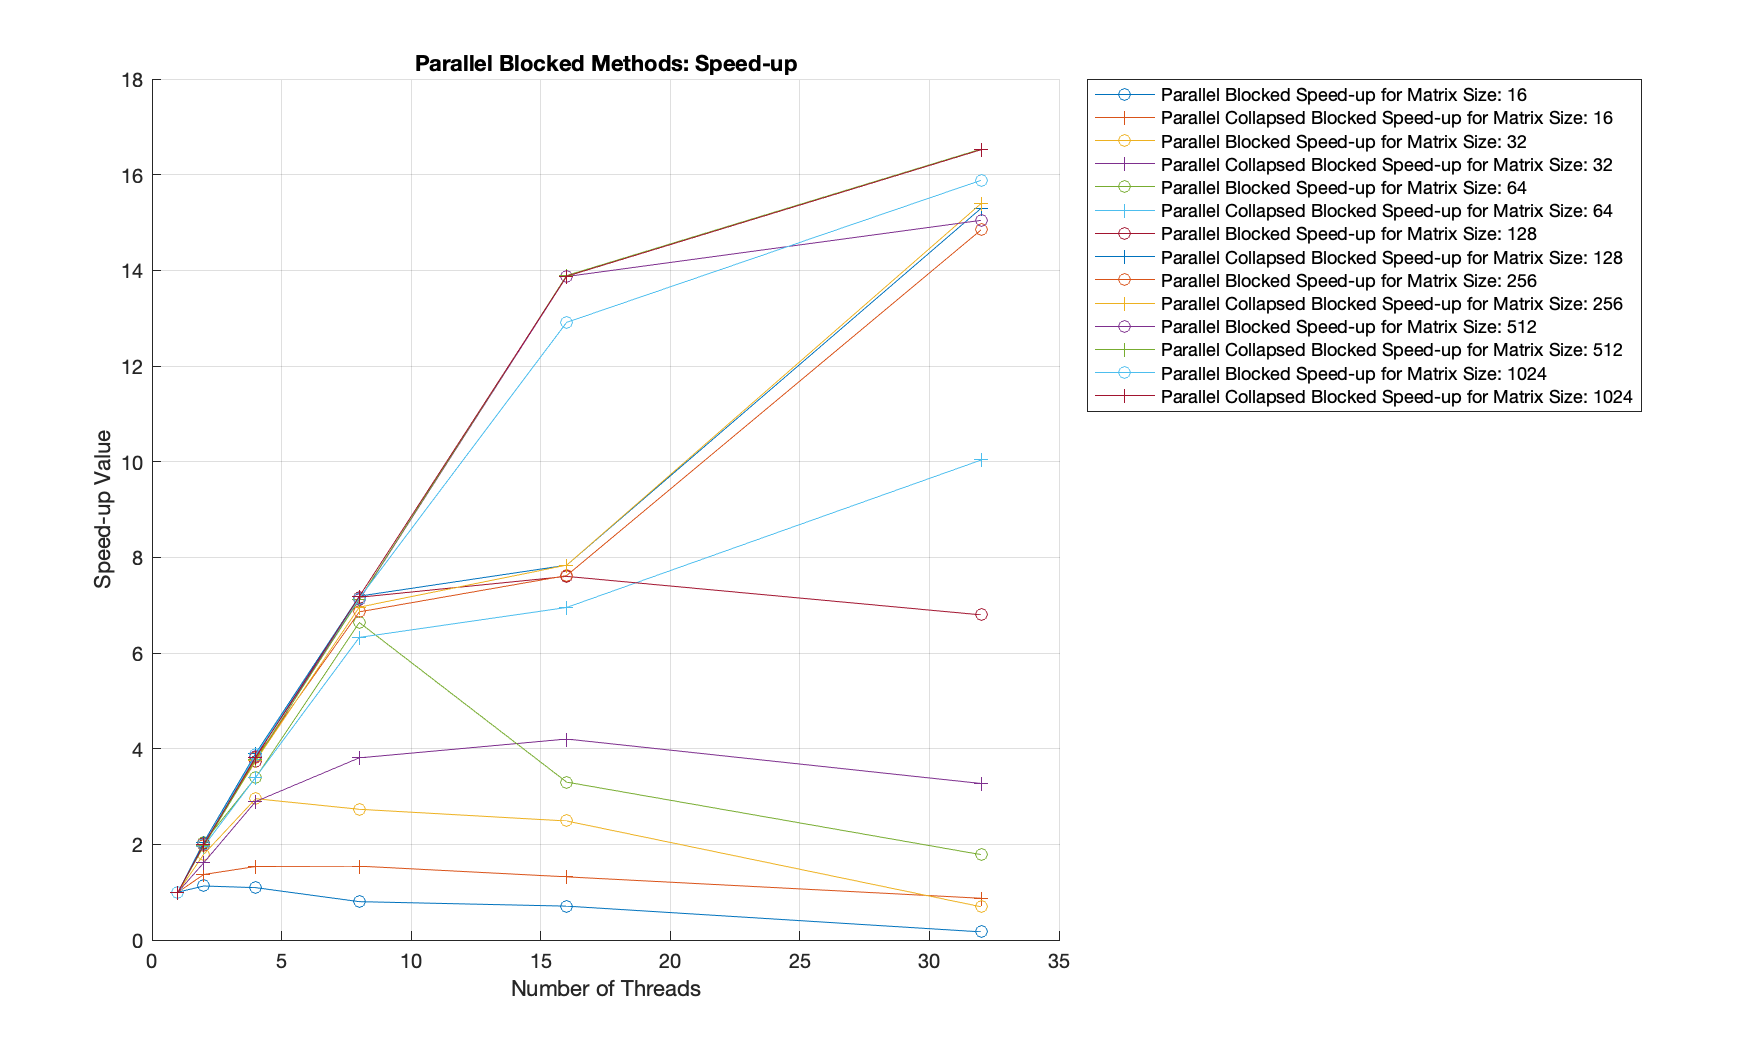
\includegraphics[width=1\linewidth]{blocked_speed-up.png}}
    \caption{Speed-up of Parallel Matmul Methods}
\end{figure}

\bigskip
\noindent
After calculating the parallel speed-up the parallel efficiency was able to be calculated as previously described. These results can be found in Table 3 and 4 for the methods using \texttt{\#pragma omp parallel for} and \texttt{\#pragma omp parallel for collapse(2)}, respectively.

\begin{table}[ht!]
    \caption{Parallel Blocked Matrix-Matrix Multiplication Efficiency}
    \centering
    \begin{tabular}{|c|c|c|c|c|c|c|}
        \hline
        \multicolumn{1}{|c|}{} & \multicolumn{6}{c|}{Number of Threads} \\
        \cline{2-7}
        \multicolumn{1}{|c|}{Matrix Size} & 1 & 2 & 4 & 8 & 16 & 32 \\
        \hline
        n = 16 & 1 & 0.5646206 & 0.2735775 & 0.1001890 & 0.0442501 & 0.0052918 \\
        \hline
        n = 32 & 1 & 0.8969649 & 0.7385930 & 0.3416050 & 0.1555109 & 0.0216836 \\
        \hline
        n = 64 & 1 & 1.0200358 & 0.8492535 & 0.8296181 & 0.2063215 & 0.0557477 \\
        \hline
        n = 128 & 1 & 1.0092099 & 0.9341466 & 0.8956708 & 0.4751154 & 0.2123936 \\
        \hline
        n = 256 & 1 & 0.9894059 & 0.9517055 & 0.8575314 & 0.4761685 & 0.4640197 \\
        \hline
        n = 512 & 1 & 0.9935669 & 0.9587436 & 0.8888089 & 0.8669076 & 0.4701788 \\
        \hline
        n = 1024 & 1 & 0.9977179 & 0.9678240 & 0.8934191 & 0.8069967 & 0.4963671 \\
        \hline
    \end{tabular}
\end{table}

\clearpage

\begin{table}[ht!]
    \caption{Parallel Collapsed Blocked Matrix-Matrix Multiplication Efficiency}
    \centering
    \begin{tabular}{|c|c|c|c|c|c|c|}
        \hline
        \multicolumn{1}{|c|}{} & \multicolumn{6}{c|}{Number of Threads} \\
        \cline{2-7}
        \multicolumn{1}{|c|}{Matrix Size} & 1 & 2 & 4 & 8 & 16 & 32 \\
        \hline
        n = 16 & 1 & 0.6851245 & 0.3840535 & 0.1930327 & 0.0825188 & 0.0272645 \\
        \hline
        n = 32 & 1 & 0.8081926 & 0.7237386 & 0.4760170 & 0.2626222 & 0.1022245 \\
        \hline
        n = 64 & 1 & 0.9812792 & 0.8501955 & 0.7907432 & 0.4344842 & 0.3135950 \\
        \hline
        n = 128 & 1 & 1.0239147 & 0.9747920 & 0.8986434 & 0.4897108 & 0.4781083 \\
        \hline
        n = 256 & 1 & 0.9969017 & 0.9357453 & 0.8698819 & 0.4897711 & 0.4812562 \\
        \hline
        n = 512 & 1 & 0.9826893 & 0.9414436 & 0.8902032 & 0.8682434 & 0.5167508 \\
        \hline
        n = 1024 & 1 & 0.9967932 & 0.9554368 & 0.8977438 & 0.8672238 & 0.5163344 \\
        \hline
    \end{tabular}
\end{table}

\bigskip
\noindent
Following these calculations, plotting the efficiency provides insight into how it changes with an increasing number of threads. This progression is depicted in Figure 2. The plot and results exhibit a decrease in parallel efficiency as the number of threads increases. However, despite the continually decreasing parallel efficiency, all the way down to 0.5 for 32 threads, it still suggests potential to further reduce computation times by increasing the number of threads. Based on this trend, increasing the thread count to 64 would reduce computation time but the improvement would be at a diminishing rate. This diminishing effect partially derives from the trade-off between faster computation speeds and managing additional overhead.

\begin{figure}[!htb]
    \centering
    \fbox{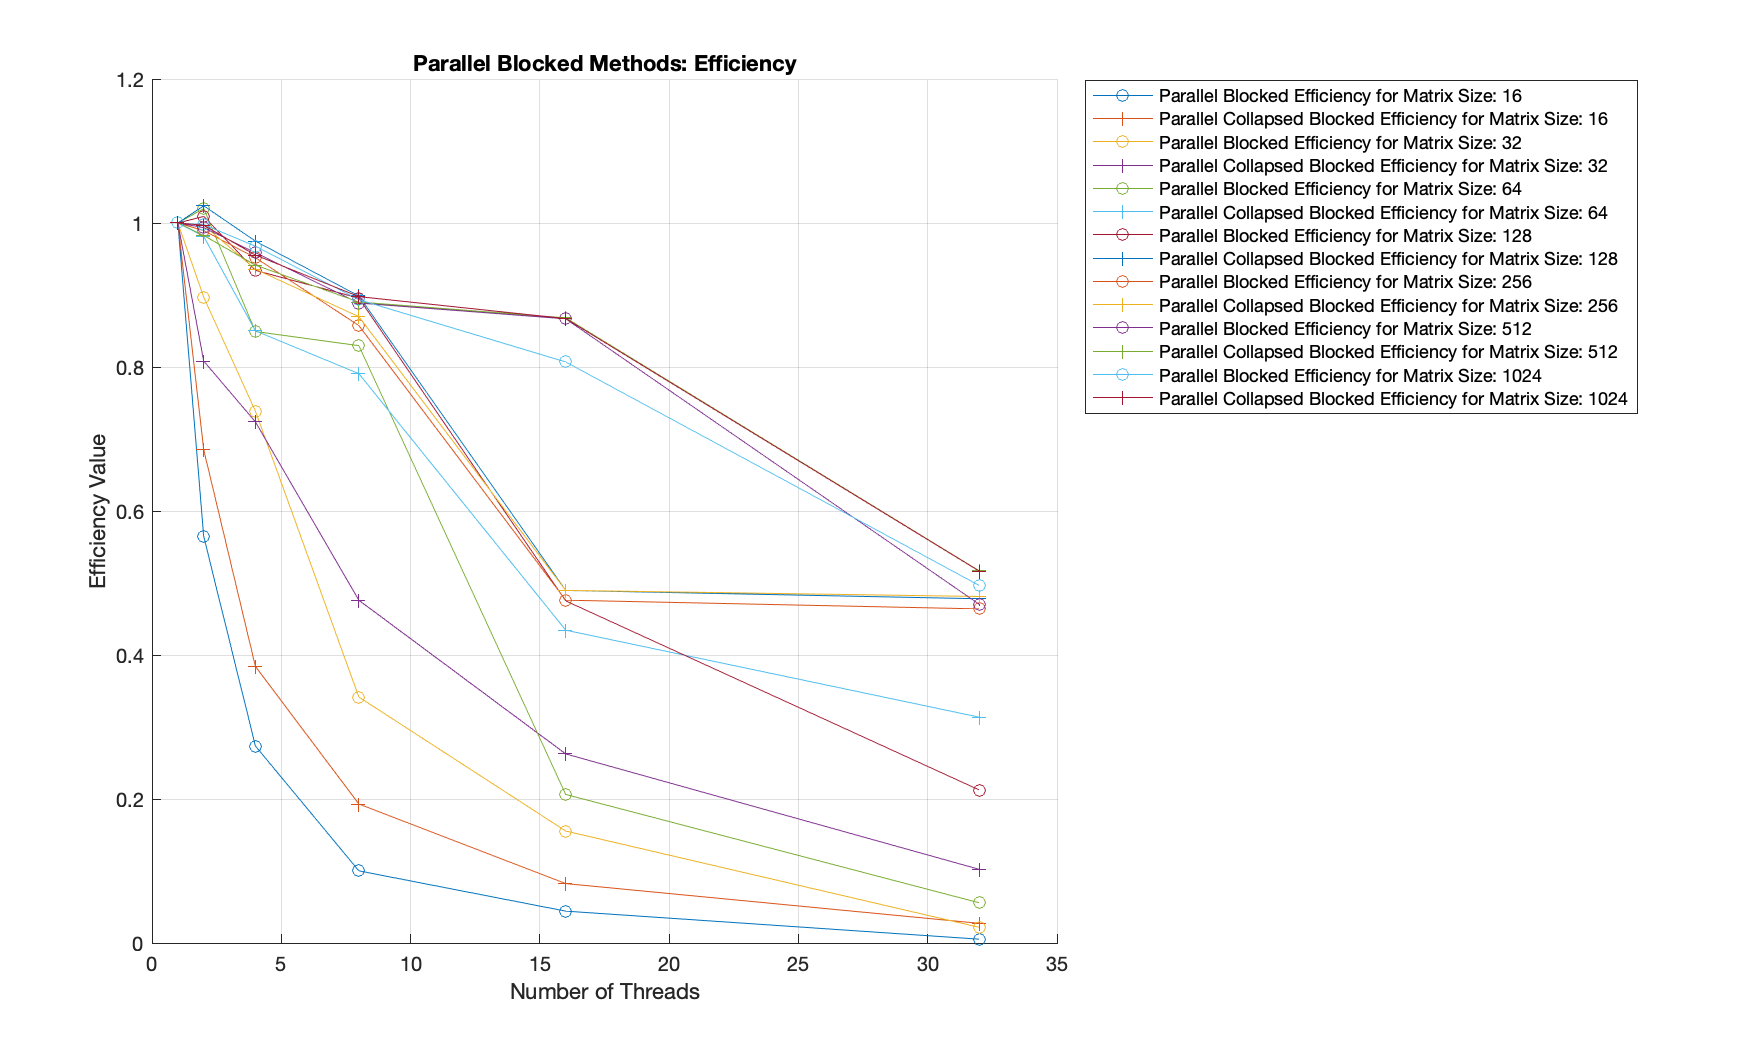
\includegraphics[width=1\linewidth]{blocked_efficiency.png}}
    \caption{Efficiency of Parallel Matmul Methods}
\end{figure}

\subsection{Matrix-Matrix Multiplication Using OpenMP Comparison}

For both blocked matmul methods the block size was set to 8 as that was the previously determined optimal block size. Given that optimal block size is contingent on hardware and the CPUs used are still Intel(R) Xeon(R) CPU E5-2650 v2 @ 2.60Hz, this will again be the optimal. By removing this additional dependency, a better comparison can be made between the implementations of using \texttt{\#pragma omp parallel for} and \texttt{\#pragma omp parallel for collapse(2)} especially with respect to their performance based on matrix size and the number of threads. 

\bigskip
\noindent
The two directives being analyzed, \texttt{\#pragma omp parallel for} and \texttt{\#pragma omp parallel for collapse(2)}, are both useful in parallelization of for loops, but complete this task differently. For the blocked matmul implementation the \texttt{\#pragma omp parallel for} directive distributes the iterations of the outer loop to the threads, which each then execute their given set. In comparison, the \texttt{\#pragma omp parallel for collapse(2)} directive, takes this approach but extends it to multiple nested loops, in this case 2. By collapsing the nested for loops into one larger iteration space, the threads can more efficiently access and utilize, essentially converting the matrix operations into "blocks" for parallel computations. 

\bigskip
\noindent
To evaluate how both directives perform based on matrix size, comparisons are made between the same thread counts to remove the influence of overhead in the results. As such, it was observed that the \texttt{collapse(2)} directive performed better for smaller matrices up to a matrix size of $n = 128$. This efficiency gain is a result to the directive's ability to better parallelize work across threads by creating a larger, more uniform iteration space. For blocked matmul this is thus quite beneficial. For larger matrices, however, the other directive has enough iterations to effectively distribute work to each thread. It is observed that the \texttt{\#pragma omp parallel for} is actually slightly faster, likely due to the reduced overhead of not having to manage the collapsed larger outer loops. 

\bigskip
\noindent
As previously mentioned, both methods exhibited a decrease in computation time as the number of threads increased. The implementation using the \texttt{collapse(2)} directive had a better parallel efficiency for smaller matrices while the thread number increased. For larger matrices, the performance between the two approaches was nearly identical, with the collapsed implementation maintaining a slight advantage. These observations highlight how important method selection is to parallel implementations. 

\section{Parallel Back Solve}
\subsection{Back Solve Algorithm for Unit Upper Triangular Matrix}
The back solve algorithm for an upper triangular matrix allows for solving the system of linear equations \(y = Ux\), where \(U\) is defined as:

\[
U =
\begin{bmatrix}
u_{11} & u_{12} & u_{13} & \cdots & u_{1n} \\
0 & u_{22} & u_{23} & \cdots & u_{2n} \\
0 & 0 & u_{33} & \cdots & u_{3n} \\
\vdots & \vdots & \vdots & \ddots & \vdots \\
0 & 0 & 0 & \cdots & u_{nn}
\end{bmatrix}
\]

\bigskip
\noindent
The resulting set of equations is as follows:

\[
\begin{aligned}
    y_{1} &= u_{11} \cdot x_{1} + u_{12} \cdot x_{2} + \cdots + u_{1n} \cdot x_{n} \\
    y_{2} &= u_{22} \cdot x_{2} + u_{23} \cdot x_{3} + \cdots + u_{2n} \cdot x_{n} \\
    y_{3} &= u_{33} \cdot x_{3} + \cdots + u_{3n} \cdots x_{n} \\
    &\vdots \\
    y_{n} &= u_{nn} \cdot x_{n}
\end{aligned}
\]

\bigskip
\noindent
From this, it can be seen that a solution can be found by beginning at the \(n^\text{th}\) equation and progressing upward to the \(1^\text{st}\). As such, from the \(n^\text{th}\) equation it can be determined that:
\[
x_{n} = \frac{y_n}{u_{nn}} \\
\]

\bigskip
\noindent
With the now known value of \(x_{n}\), the \(n-1^{\text{th}}\) equation, \(y_{n-1} = u_{n-1,n-1} \cdot x_{n-1} + u_{n-1,n} \cdot {x_n}\), only has the one unknown of \(x_{n-1}\). Back solving for this value, it is found that:

\[
x_{n-1} = \frac{y_{n-1} - u_{n-1,n} \cdot {x_n}}{u_{n-1,n-1}}
\]

\bigskip
\noindent
After determining the value of the first unknown $x_{n}$, this process of using the solutions from the previous equations for solving can be generalized to:

\[
x_{i} = \frac{y_{i} - \sum\limits_{j=i+1}^{n} u_{ij} \cdot x_{j}}{u_{ii}} \quad \forall i = n-1, \cdots, 1
\]

\bigskip 
\noindent
Given that the matrix of interest is unit upper triangular, the matrix elements $u_{ij} = 1$ if $i = j$ which occurs along the diagonal. As such the procedure can be simplified to:
\[
x_{i} = y_{i} - \sum\limits_{j=i+1}^{n} u_{ij} \cdot x_{j}\quad \forall i = n-1, \cdots, 1
\]

\bigskip
\noindent
At this point all the required steps for the back solve algorithm have been laid out. Thus the back solve algorithm is:

\begin{algorithm}[hbt!]
\caption{Back Solve for Unit Upper Triangular Matrix}
\label{algo:back_substitution}
\SetAlgoLined
\KwData{Unit upper triangular matrix $U$, vector $y$, dimension $n$}
\KwResult{Solution vector $x$}
Initialize $x$ as an array of length $n$\;
$x[n] \gets y[n]$ \;
\For{$i \gets n-1$ \KwTo $1$}{
    $sum \gets 0$\;
    \For{$j \gets i+1$ \KwTo $n$}{
        $sum \gets sum + U[i][j] \times x[j]$\;
    }
    $x[i] \gets y[i] - sum$\;
}
\Return $x$\;
\end{algorithm}

\subsection{Parallelization of the Back Solve Algorithm}
In Algorithm 1, parallelization can be applied to the inner loop responsible for updating the sum. By having each thread independently complete an iteration of computing the product of \( U[i][j]\) with $x[j]$ and then add it to the sum, the algorithm efficiently uses parallel computation to solve for $x_{i}$. However, with this approach there is a risk of potential race conditions when multiple threads attempt to update the sum at the same time. To avoid this problem a \texttt{reduction(+:sum)} directive can be introduced to ensure safe threading. An alternative approach is to restructure how the newly computed value of $x_{i}$ is used for the subsequent updates of the \(x\) vector. Rather than updating each vector element by utilizing all previous known values, which poses a potential problem, instead the new $x_{i}$ value can be used to update all the other elements in the vector concurrently. This adjustment leads to updates occurring now column-wise instead of row-wise. This improvement both guarantees that each vector element is only modified by a single thread at any time while improving efficiency of the method. The details for this parallelized version are provided in Algorithm 2.
\clearpage

\begin{algorithm}[hbt!]
\caption{Back Solve for Unit Upper Triangular Matrix}
\label{algo:back_substitution}
\SetAlgoLined
\KwData{Unit upper triangular matrix $U$, vector $y$, dimension $n$}
\KwResult{Solution vector $x$}
Initialize $x$ as a zero vector of length $n$\;
\For{$j \gets n-1$ \KwTo $0$}{
    $x[j] \gets x[j] + y[j]$ \;
    \textbf{Parallel} \For{$i \gets 0$ \KwTo $j$}{
        $x[i] \gets x[i] - U[i][j] \times x[j]$\;
    }
}
\Return $x$\;
\end{algorithm}

\subsection{Parallel Back Solve with a Unit Upper Triangular Matrix and Static Scheduling Timing}

\begin{table}[ht!]
    \caption{Parallel Back Solve with Static Scheduling Timings (Seconds) on NOTS}
    \centering
    \resizebox{\textwidth}{!}{%
    \begin{tabular}{|c|c|c|c|c|c|c|}
        \hline
        \multicolumn{1}{|c|}{} & \multicolumn{6}{c|}{Number of Threads} \\
        \cline{2-7}
        \multicolumn{1}{|c|}{Matrix Size} & 1 & 2 & 4 & 8 & 16 & 32 \\
        \hline
        n = 16 & 8.20011e-07 & 6.7085e-07 & 6.88061e-07 & 7.69421e-07, & 9.65372e-07 & 1.28314e-06 \\
        \hline
        n = 32 & 2.22504e-06 & 2.56002e-06 & 2.87123e-06 & 2.58096e-06 & 3.13871e-06 & 6.07774e-06 \\
        \hline
        n = 64 & 8.39047e-06 & 8.35247e-06 & 8.60311e-06 & 9.59463e-06 & 9.29609e-06 & 1.74093e-05 \\
        \hline
        n = 128 & 3.32709e-05 & 3.20963e-05 & 3.3632e-05 & 3.58845e-05 & 5.70576e-05 & 5.43984e-05 \\
        \hline
        n = 256 & 0.000178044 & 0.000174087 & 0.000186581 & 0.000175001 & 0.000176746 & 0.000190061 \\
        \hline
        n = 512 & 0.000735507 & 0.000758221 & 0.000833904 & 0.000762215 & 0.000771164 & 0.000852399 \\
        \hline
        n = 1024 & 0.00306181 & 0.00287781 & 0.00297813 & 0.00294556 & 0.00304278 & 0.0030443 \\
        \hline
    \end{tabular}
    }
\end{table}

\subsection{Parallel Back Solve with a Unit Upper Triangular Matrix and Dynamic Scheduling Timing}

\begin{table}[ht!]
    \caption{Parallel Back Solve with Dynamic Scheduling Timings (Seconds) on NOTS}
    \centering
    \resizebox{\textwidth}{!}{%
    \begin{tabular}{|c|c|c|c|c|c|c|}
        \hline
        \multicolumn{1}{|c|}{} & \multicolumn{6}{c|}{Number of Threads} \\
        \cline{2-7}
        \multicolumn{1}{|c|}{Matrix Size} & 1 & 2 & 4 & 8 & 16 & 32 \\
        \hline
        n = 16 & 4.59924e-06 & 5.10991e-06 & 4.5462e-06 & 5.3139e-06 & 5.26503e-06 & 7.73981e-06 \\
        \hline
        n = 32 & 1.91147e-05 & 1.28318e-05 & 1.33979e-05 & 1.48906e-05 & 1.43745e-05 & 2.14069e-05 \\
        \hline
        n = 64 & 4.27759e-05 & 4.29252e-05 & 4.63497e-05 & 4.65312e-05 & 4.88424e-05 & 5.17755e-05 \\
        \hline
        n = 128 & 0.000173092 & 0.000161693 & 0.000162513 & 0.00016506 & 0.000168359 & 0.000167735 \\
        \hline
        n = 256 & 0.000910005 & 0.000915316 & 0.00091138 & 0.000915389 & 0.000905255 & 0.000919714 \\
        \hline
        n = 512 & 0.00397152 & 0.00395695 & 0.00396906 & 0.0040007 & 0.00407617 & 0.00403947 \\
        \hline
        n = 1024 & 0.0154925 & 0.0148775 & 0.0148746 & 0.0149279 & 0.0155612 & 0.01547464 \\
        \hline
    \end{tabular}
    }
\end{table}

\subsection{Static Versus Dynamic Scheduling}
The performance of parallel back solve with a unit upper triangular matrix and dynamic scheduling was consistently slower than the static scheduling version, often by an order of magnitude. This makes sense when observing where the parallelization occurs in the implementation and how the scheduler assigns threads to handle it based on scheduling type. For the static scheduling, each thread is given a fixed number of for loop iterations at the beginning of the parallel region. This is desirable when each iteration takes about the same time, avoiding a workload imbalance. The dynamic scheduler, on the other hand, is desirable when there is a variance in how long each iteration takes as it dynamically allocates iterations to minimize the unequal distribution of work. However, this flexibility produces a significant overhead. In cases like the parallel back solve where the workload per iteration is uniform\textemdash one multiplication and one addition\textemdash the dynamic scheduler only adds unnecessary overhead and reduces performance. This behavior aligns with what was observed in the results and emphasizes the importance of correctly choosing schedulers based on problem requirements.

\subsection{Parallel Back Solve Efficiency}
The calculation of the parallel efficiency of the back solve implementations with static and dynamic scheduling followed the same process as previously described. As such, the resulting efficiency values can be found in Table 7 and Table 8 respectively.

\begin{table}[ht!]
    \caption{Parallel Back Solve with Static Scheduling Efficiency}
    \centering
    \begin{tabular}{|c|c|c|c|c|c|c|}
        \hline
        \multicolumn{1}{|c|}{} & \multicolumn{6}{c|}{Number of Threads} \\
        \cline{2-7}
        \multicolumn{1}{|c|}{Matrix Size} & 1 & 2 & 4 & 8 & 16 & 32 \\
        \hline
        n = 16 & 1 & 0.6111731 & 0.2979426 & 0.2979426 & 0.0530890 & 0.0199708 \\
        \hline
        n = 32 & 1 & 0.4345747 & 0.1937357 & 0.1077622 & 0.0443064 & 0.0114405 \\
        \hline
        n = 64 & 1 & 0.5022747 & 0.2438208 & 0.1093120 & 0.0564112 & 0.0150610 \\
        \hline
        n = 128 & 1 & 0.5182980 & 0.2473158 & 0.1158957 & 0.0364444 & 0.0191129 \\
        \hline
        n = 256 & 1 & 0.5113650 & 0.2385612 & 0.1271735 & 0.0629589 & 0.0292741 \\
        \hline
        n = 512 & 1 & 0.4850215 & 0.2205011 & 0.1206200 & 0.0596101 & 0.0269645 \\
        \hline
        n = 1024 & 1 & 0.5319687 & 0.2570245 & 0.1299332 & 0.0628908 & 0.0314297 \\
        \hline
    \end{tabular}
\end{table}

\begin{table}[ht!]
    \caption{Parallel Back Solve with Dynamic Scheduling Efficiency}
    \centering
    \begin{tabular}{|c|c|c|c|c|c|c|}
        \hline
        \multicolumn{1}{|c|}{} & \multicolumn{6}{c|}{Number of Threads} \\
        \cline{2-7}
        \multicolumn{1}{|c|}{Matrix Size} & 1 & 2 & 4 & 8 & 16 & 32 \\
        \hline
        n = 16 & 1 & 0.4500314 & 0.2529167 & 0.1081889 & 0.0545965 & 0.0185697 \\
        \hline
        n = 32 & 1 & 0.7448175 & 0.3566734 & 0.1604594 & 0.0831102 & 0.0279038 \\
        \hline
        n = 64 & 1 & 0.4982609 & 0.2307237 & 0.1149118 & 0.0547371 & 0.0258181 \\
        \hline
        n = 128 & 1 & 0.5352488 & 0.2662740 & 0.1310826 & 0.0642570 & 0.0322480 \\
        \hline
        n = 256 & 1 & 0.4970988 & 0.2496228 & 0.1242647 & 0.0628279 & 0.0309201 \\
        \hline
        n = 512 & 1 & 0.5018410 & 0.2501549 & 0.1240882 & 0.0608953 & 0.0307243 \\
        \hline
        n = 1024 & 1 & 0.5206687 & 0.2603851 & 0.1297277 & 0.0622240 & 0.0312861 \\
        \hline
    \end{tabular}
\end{table}

\bigskip
\noindent
The parallel efficiency of the implementations as a function of block size can also be seen in Figure 3 for the static scheduled version and Figure 4 for the dynamic scheduled version.

\clearpage

\begin{figure}[htb!]
    \centering
    \fbox{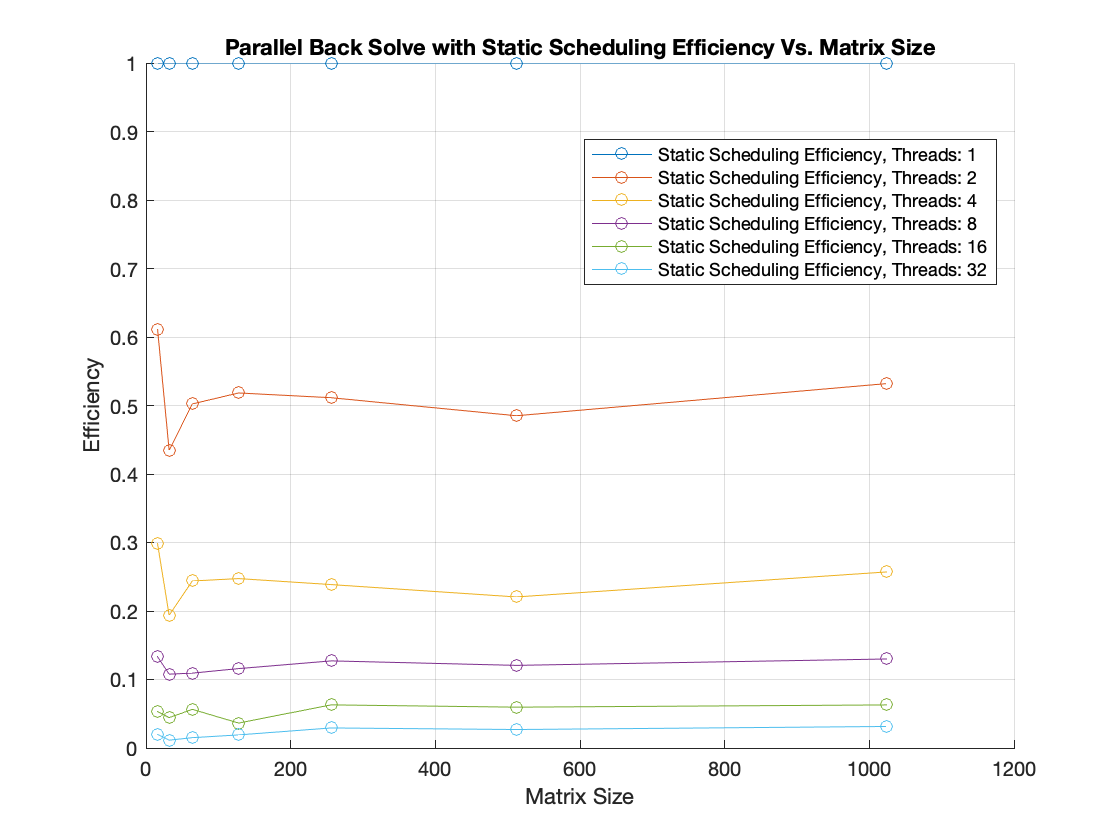
\includegraphics[width=0.7\linewidth]{static_efficiency.png}}
    \caption{Efficiency of Parallel Back Solve with Static Scheduling}
\end{figure}

\begin{figure}[htb!]
    \centering
    \fbox{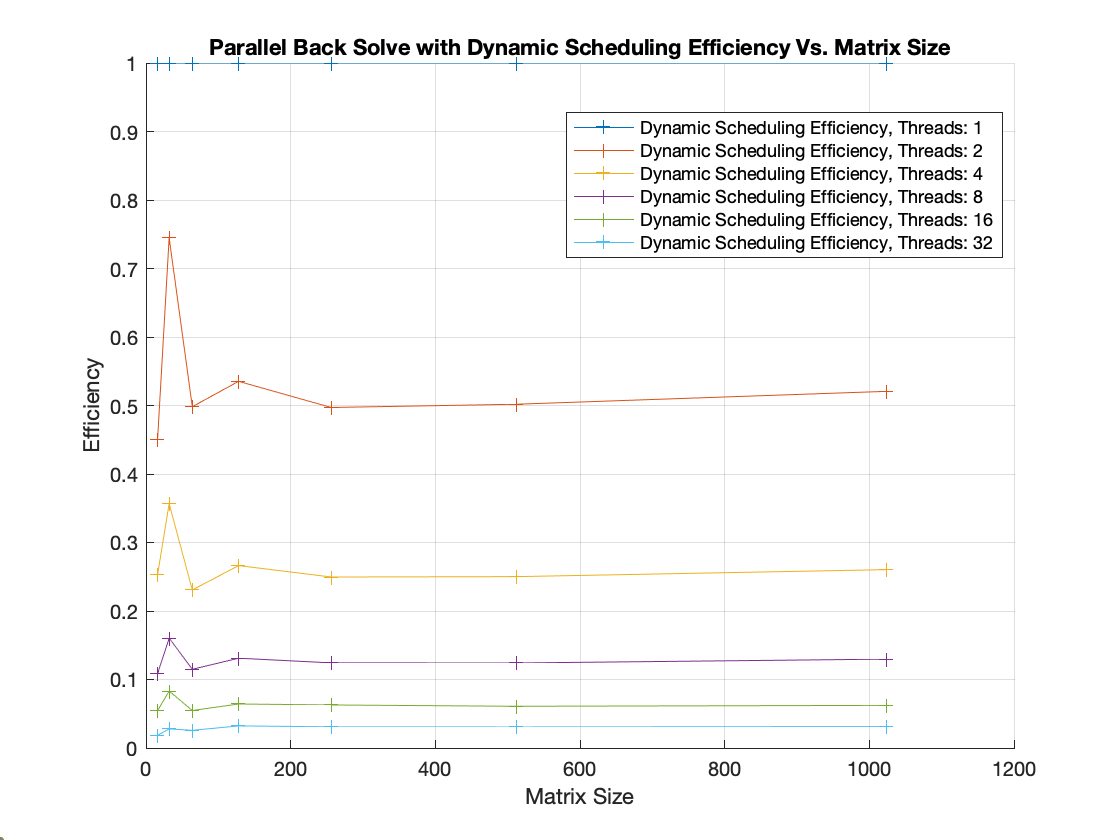
\includegraphics[width=0.7\linewidth]{dynamic_efficiency.png}}
    \caption{Efficiency of Parallel Back Solve with Dynamic Scheduling}
\end{figure}

\clearpage

\subsection{Parallel Efficiency Discussion}
As illustrated in Figure 3 and 4, for the same matrix size the parallel efficiency continues to decline with an increase in number of threads. This is directly a result of the overhead of OpenMP and the fact that this problem structure does not scale well with threading. A detailed examination of the parallel back solve implementation reveals that, across all the instances, the optimal thread count is between 1 and 4. This observation suggests a fundamental mismatch between the problem structure and the advantages offered by parallelization. Even with larger matrices the gains from more threads are not observed. At 32 threads, the parallel efficiency drops below 0.05, indicating that additional threads fail to add any enhancements in performance. These diminishing returns are exhibited as early as 8 threads, suggesting to avoid going above a small number of threads. In order to make parallelization a feasible option to scale for parallel back solve implementations significant work is required to reduce overhead and likely would require a overhaul of the method.  


\subsection{Parallel Back Solve with Bidiagonal Matrix}
If the triangular matrix is reduced to a bidiagonal form, it is expected that the parallel efficiency would decline with an increase in the number of threads. The primary issue lies in the functionally eliminated opportunity for parallelization. In the bidiagonal scenario, the calculation of $x_{i}$ where the parallelization was utilized simplifies to $x_{i} = y_{i} - u_{i,i+1} \cdot x_{i+1}, \forall i = n-1, \ldots, 1$, with $x_{n} = y_{n}$ known. Consequently, the parallel for loop becomes singular in its task execution, resulting in any additional threads useless. As such, adding more threads only harms performance as it produces more overhead and slowing the implementation time. Given that parallel efficiency is $E(n) = \frac{S(n)}{n}$ and the speed-up is $S(n) = \frac{T(1)}{T(n)}$, the behavior of the parallel efficiency is dependent on $S(n)$ and $n$. Given that parallelization does not benefit the method implementation it is not expected that $T(n) < T(1)$, with in reality $T(n)$ likely much larger due to the additional overhead caused by threads. Compounding on this, the parallel efficiency $E(n)$ will only get worse as it is divided by the growing number of processors. In conclusion, parallelization for this matrix structure and problem offers no advantage and instead a completely serial implementation is expected to be the fastest as it does not introduce overhead compared to a threading version.

\end{document}


